\fsection{Esquema de la instalación}
\fsubsection{Disposición de la mesa de trabajo}
La celda se monta sobre una mesa móvil con ruedas de 1400 × 800 mm. En el lado izquierdo está el contenedor con
las piezas mezcladas, el robot se fija en la parte delantera, centrado a lo largo de la mesa, y a su alrededor se reparten las bandejas de
colocación. La cámara está fija sobre el contenedor de piezas.

En este proyecto todas las piezas del contenedor tienen características similares, por lo que el robot las
deposita todas en una única bandeja de colocación (bandeja 1). Las bandejas 2 y 3 quedan reservadas para la
ampliación de clasificación por tipo de pieza descrita en el apartado de posibles ampliaciones.

\begin{figure}[H]
	\centering
	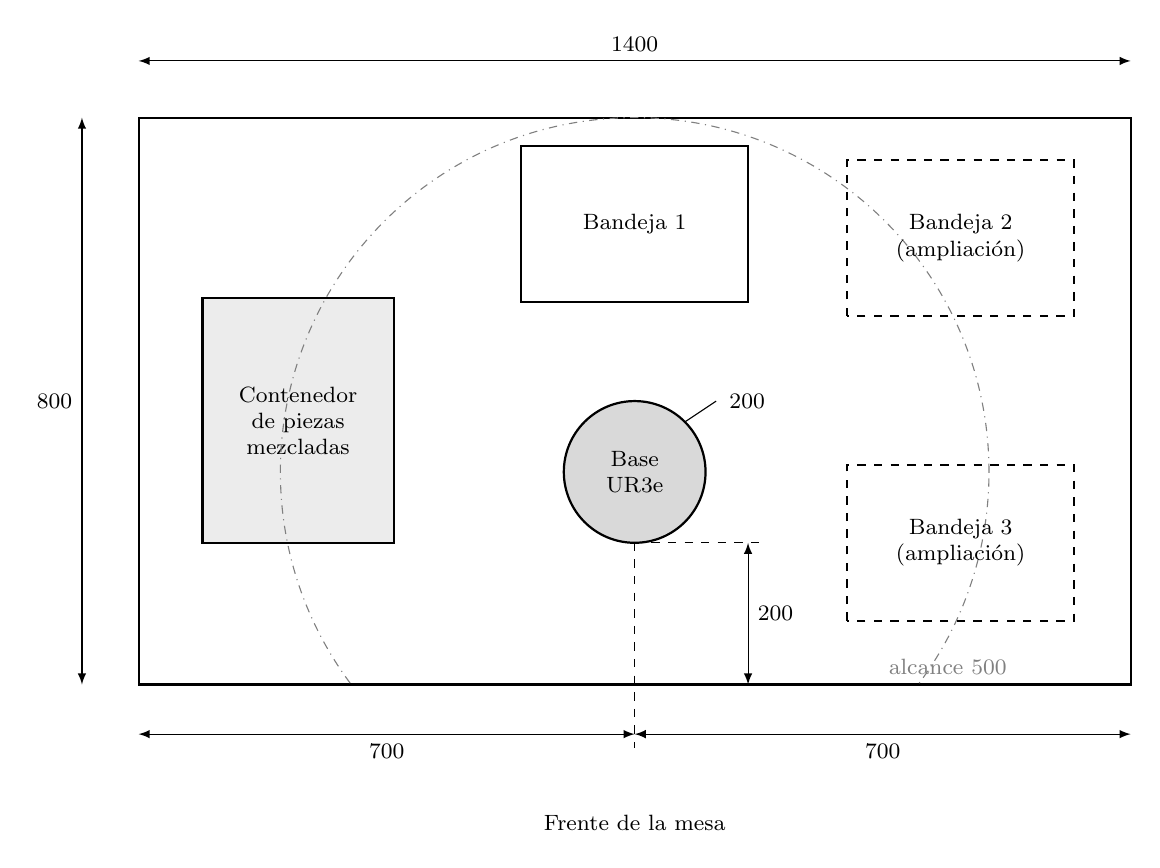
\begin{tikzpicture}[x=0.09mm, y=0.09mm,
			cota/.style={latex-latex, thin},
			etiqueta/.style={font=\footnotesize, align=center},
		]
		% mesa
		\draw[thick] (0,0) rectangle (1400,800);
		% contenedor de piezas (345 x 270 exterior)
		\draw[thick, fill=gray!15] (90,200) rectangle (360,545);
		\node[etiqueta] at (225,372) {Contenedor\\de piezas\\mezcladas};
		% base del robot (placa de montaje Ø200), centrada en la mesa
		\draw[thick, fill=gray!30] (700,300) circle (100);
		\node[etiqueta] at (700,300) {Base\\UR3e};
		% alcance del UR3e (500 mm)
		\begin{scope}
			\clip (0,0) rectangle (1400,800);
			\draw[thin, dash dot, gray] (700,300) circle (500);
		\end{scope}
		\node[etiqueta, gray, anchor=south west] at (1045,0) {alcance 500};
		% bandejas de colocación
		\draw[thick] (540,540) rectangle (860,760);
		\draw[thick, dashed] (1000,520) rectangle (1320,740);
		\draw[thick, dashed] (1000,90) rectangle (1320,310);
		\node[etiqueta] at (700,650) {Bandeja 1};
		\node[etiqueta] at (1160,630) {Bandeja 2\\(ampliación)};
		\node[etiqueta] at (1160,200) {Bandeja 3\\(ampliación)};
		% cotas
		\draw[cota] (0,880) -- node[above, etiqueta] {1400} (1400,880);
		\draw[cota] (-80,0) -- node[left, etiqueta] {800} (-80,800);
		\draw[cota] (860,0) -- node[right, etiqueta] {200} (860,200);
		\draw[thin, dashed] (700,200) -- (880,200);
		\draw[cota] (0,-70) -- node[below, etiqueta] {700} (700,-70);
		\draw[cota] (700,-70) -- node[below, etiqueta] {700} (1400,-70);
		\draw[thin, dashed] (700,200) -- (700,-90);
		\node[etiqueta, anchor=west] at (820,400) {$\varnothing$200};
		\draw[thin] (770,370) -- (815,400);
		\node[etiqueta, anchor=north] at (700,-170) {Frente de la mesa};
	\end{tikzpicture}
	\caption{Disposición de la mesa de trabajo, vista en planta (cotas en mm; la posición de las bandejas es orientativa). Las bandejas en línea discontinua están reservadas para la ampliación. La línea de puntos y rayas indica el alcance aproximado del UR3e.}
\end{figure}

\fsubsection{Esquema de comunicaciones}
La siguiente figura muestra los equipos de la celda y cómo se conectan entre sí.

\begin{figure}[H]
	\centering
	\begin{tikzpicture}[
			node distance=1cm and 0.6cm,
			equipo/.style={draw, rounded corners, thick, align=center, minimum width=3.2cm, minimum height=1.2cm, font=\small},
			fisico/.style={draw, dashed, align=center, minimum width=2.4cm, minimum height=0.9cm, font=\small},
			red/.style={thick},
			mec/.style={-latex, dashed},
		]
		\node[equipo] (sw) {Red Profinet\\\footnotesize 192.168.15.xxx};
		\node[equipo, above left=of sw] (cam) {Cámara 3D\\Orbbec Femto Mega\\\footnotesize 192.168.15.41};
		\node[equipo, above right=of sw] (ipc) {IPC SIMATIC BX-59A\\Robot Pick AI (Docker)\\\footnotesize 192.168.15.19};
		\node[equipo, below left=of sw] (plc) {PLC S7-1500\\1516-3 PN/DP V2.9\\\footnotesize 192.168.15.10};
		\node[equipo, below right=of sw] (ur) {Robot UR3e\\\footnotesize 192.168.15.20};

		\draw[red] (cam) -- (sw);
		\draw[red] (ipc) -- (sw);
		\draw[red] (plc) -- (sw);
		\draw[red] (ur) -- (sw);

		\node[equipo, below=of sw] (pc) {PC de ingeniería\\TIA Portal V18\\\footnotesize 192.168.15.xxx};
		\draw[red] (pc) -- (sw);

		\node[equipo, below=of ur] (tool) {Pinza de vacío\\OnRobot VGC10};
		\draw[red] (ur) -- node[right, font=\footnotesize] {E/S herramienta} (tool);

		\node[fisico, below=of plc] (bin) {Contenedor de\\piezas (desordenado)};
		\node[fisico, below=0.6cm of tool] (out) {Bandeja de colocación};

		\draw[mec] (cam.west) to[bend right=30] node[right, font=\footnotesize, align=center] {imagen\\y nube de puntos} (bin.west);
		\draw[mec] (bin) -- node[above, font=\footnotesize] {agarre} (tool);
		\draw[mec] (tool) -- node[right, font=\footnotesize] {depósito} (out);
	\end{tikzpicture}
	\caption{Esquema de bloques de la celda: red de comunicaciones (línea continua) y flujo físico de las piezas (línea discontinua).}
\end{figure}

El ciclo de trabajo es el siguiente: el PLC pide al IPC la siguiente pieza; el IPC analiza la imagen de la
cámara con el modelo de IA y devuelve las coordenadas del punto de agarre; el PLC se las pasa al robot, que
recoge la pieza con la pinza de vacío y la deja en la bandeja de colocación. Cuando el contenedor queda vacío, el IPC lo notifica y el ciclo se detiene.
